% Created 2019-11-18 Mon 12:59
% Intended LaTeX compiler: pdflatex
\documentclass[11pt]{article}
\usepackage[utf8]{inputenc}
\usepackage[T1]{fontenc}
\usepackage{graphicx}
\usepackage{grffile}
\usepackage{longtable}
\usepackage{wrapfig}
\usepackage{rotating}
\usepackage[normalem]{ulem}
\usepackage{amsmath}
\usepackage{textcomp}
\usepackage{amssymb}
\usepackage{capt-of}
\usepackage{hyperref}
\usepackage{minted}
\usepackage[margin=0.75in]{geometry}
\renewcommand{\familydefault}{\sfdefault}
\usepackage{xcolor}
\usepackage{fancyhdr}
\pagestyle{fancyplain}
\chead{Assignment 3 - Practical Statistics with R}
\lhead{Guilherme G. Haetinger}
\rhead{Fall 2019}
\usemintedstyle{friendly}
\author{Guilherme Gomes Haetinger}
\date{\today}
\title{\huge Assignment 3}
\hypersetup{
 pdfauthor={Guilherme Gomes Haetinger},
 pdftitle={\huge Assignment 3},
 pdfkeywords={},
 pdfsubject={},
 pdfcreator={Emacs 27.0.50 (Org mode 9.2.6)}, 
 pdflang={English}}
\begin{document}

\maketitle
\thispagestyle{empty}

\noindent\rule{\textwidth}{0.5pt}

\section{\underline{True or False}}
\label{sec:orgd26d85e}

\subsection{If a fair coin is tossed many times and the last eight tosses are all heads, then the chance that the next toss will be heads is somewhat less than 50\%.}
\label{sec:org118ecb7}
\colorbox{yellow}{False} \(\to\) The tosses are independent, meaning the outcome of previous events don't have any effect on the result of the following events.
\subsection{Drawing a face card (jack, queen, or king) and drawing a red card from a full deck of playing cards are mutually exclusive events.}
\label{sec:orgc3ce876}
\colorbox{yellow}{False} \(\to\) They can both happen, because a card can be both a face card and a red card.
\subsection{Drawing a face card and drawing an ace from a full deck of playing cards are mutually exclusive events.}
\label{sec:orgbc3fa68}
\colorbox{yellow}{True} \(\to\) A card can't be both an ace card and a face card.

\noindent\rule{\textwidth}{0.5pt}

\section{\underline{Roulette Wheel}}
\label{sec:orgd464ee6}
The game of roulette involves spinning a wheel with 38 slots: 18 red, 18 black, and 2 green. A ball is spun onto the wheel and will eventually land in a slot, where each slot has an equal chance of capturing the ball.
\subsection{You watch a roulette wheel spin 3 consecutive times and the ball lands on a red slot each time. What is the probability that the ball will land on a red slot on the next spin?}
\label{sec:orgbddc2e4}
The probability is the same as before the spins. This means the probability will be \(\frac{18}{38}\).
\subsection{You watch a roulette wheel spin 300 consecutive times and the ball lands on a red slot each time. What is the probability that the ball will land on a red slot on the next spin?}
\label{sec:org77499b9}
Considering that the wheel is trustworthy, the probability is still the same.
\subsection{Are you equally confident of your answers to parts (a) and (b)? Why or why not?}
\label{sec:org2631391}
Answer (b) doesn't express much confidence since the chances that the ball lands 300 times consecutively is pretty low (\(\frac{18}{38}^{300}\)). The same thing can't be said for answer (a), since it's way more probable.

\noindent\rule{\textwidth}{0.5pt}

\section{\underline{Coin flips}}
\label{sec:orgd1a8453}
If you flip a fair coin 10 times, what is the probability of
\subsection{Getting all tails?}
\label{sec:org6c5b4b4}
We need 10 times the same outcome of independent events: \(P(A)*P(B)*P(C)*... = 0.5^{10}\)

\begin{minted}[,bgcolor=lightgray]{r}
dbinom(0, 10, .5)
\end{minted}

\begin{verbatim}
0.0009765625
\end{verbatim}

\subsection{Getting all heads?}
\label{sec:orgba31a6c}
The probability of heads is the same as tails, so it's the same answer.

\begin{minted}[,bgcolor=lightgray]{r}
dbinom(10, 10, .5)
\end{minted}

\begin{verbatim}
0.0009765625
\end{verbatim}

\subsection{Get at least one tails?}
\label{sec:org390a75d}
The probability will be \(1 - P(10 heads)\).

\begin{minted}[,bgcolor=lightgray]{r}
1 - pbinom(0, 10, .5)
\end{minted}

\begin{verbatim}
0.9990234375
\end{verbatim}


\noindent\rule{\textwidth}{0.5pt}
\section{\underline{Dice rolls}}
\label{sec:org793ed78}
If you roll a pair of fair dice, what is the probability of

\begin{minted}[,bgcolor=lightgray]{r}
size <- 1:6
first <- sample(size, 10000, replace=TRUE)
second <- sample(size, 10000, replace=TRUE)

summation <- first + second
\end{minted}

\subsection{getting a sum of 1?}
\label{sec:orge760101}
\begin{enumerate}
\item There is no 0s on a regular dice.
\end{enumerate}

\begin{minted}[,bgcolor=lightgray]{r}
length(summation[summation == 1])/10000
\end{minted}

\begin{verbatim}
0
\end{verbatim}

\subsection{getting a sum of 5?}
\label{sec:org8efb85a}
We have 36 possibilities of sums. From these, only \(4+1, 1+4, 3+2, 2+3\) fill this condition. So \(\frac{4}{36}\).

\begin{minted}[,bgcolor=lightgray]{r}
length(summation[summation == 5])/10000
\end{minted}

\begin{verbatim}
0.106
\end{verbatim}

\subsection{getting a sum of 12?}
\label{sec:org89549f7}
1 out of the 36.

\begin{minted}[,bgcolor=lightgray]{r}
length(summation[summation == 12])/10000
\end{minted}

\begin{verbatim}
0.0279
\end{verbatim}


\noindent\rule{\textwidth}{0.5pt}
\section{\underline{Swing voters}}
\label{sec:org8043e99}
A Pew Research survey asked 2,373 randomly sampled registered voters their political affiliation (Republican, Democrat, or Independent) and whether or not they identify as swing voters. 35\% of respondents identified as Independent, 23\% identified as swing voters, and 11\% identified as both.
\subsection{Are being Independent and being a swing voter disjoint, i.e. mutually exclusive?}
\label{sec:org416f4ae}
No, since we have \emph{11\%} of identification to both classes.
\subsection{Draw a Venn diagram summarizing the variables and their associated probabilities.}
\label{sec:org099194e}
\begin{minted}[,bgcolor=lightgray]{r}
library(VennDiagram)
draw.triple.venn(area1 = 35, area2 = 23, area3 = 100,
                 n12 = 11, n13 = 35, n23 = 23, n123 = 11,
                 category = c("Independent", "Swing", "All"),
                 fill = c("green", "blue", "orange")
                 )
\end{minted}

\begin{center}
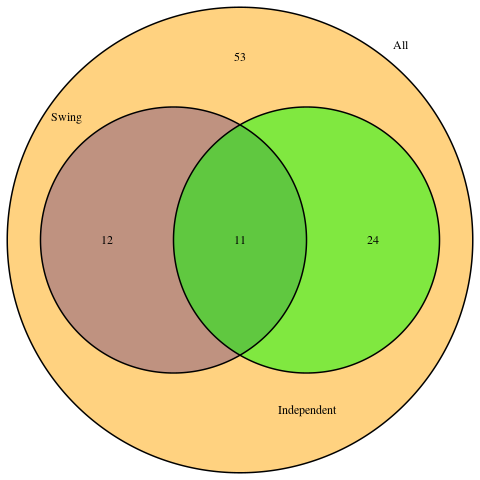
\includegraphics[width=.9\linewidth]{venn.png}
\end{center}

\subsection{What percent of voters are Independent but not swing voters?}
\label{sec:org430438c}
The sample contains a total of \emph{35\% + 23\% - 11\% = 47\%} people who answered the specific sets. This way, we know that \(I + S - (I \cap S) - S =\) \emph{47\% - 23\% = 24\%}. 
\subsection{What percent of voters are Independent or swing voters?}
\label{sec:org0f7b70f}
The same way we did the previous, we know \emph{47\% - 35\% = 12\%}.
\subsection{What percent of voters are neither Independent nor swing voters?}
\label{sec:org146cb02}
We have \emph{47\%} containing the answers we accounted. Therefore, there are \emph{53\%} that didn't answer to be Independent or swing voters.
\subsection{Is the event that someone is a swing voter independent of the event that someone is a political Independent?}
\label{sec:org6cf97bc}
I don't see how it would be. Considering that less than half of the independent set is also a swing voter, knowing that someone is a political independent can make us guess that they aren't swing voters.
\section{\underline{Disjoint vs. Independent}}
\label{sec:org4e74d27}
In parts (a) and (b), identify whether the events are disjoint, independent, or neither (events cannot be both disjoint and independent).
\subsection{You and a randomly selected student from your class both earn A's in this course.}
\label{sec:org13c333b}
\colorbox{yellow}{Independent} \(\to\) The outcome of my exam doesn't have any influence in another random student's.
\subsection{You and your class study partner both earn A's in this course.}
\label{sec:orgb5a3111}
\colorbox{yellow}{Neither} \(\to\) The outcome is influenced, considering we prepared together and are expected to have the same amount of knowledge for the exam. They can happen at the same time.
\subsection{If two events can occur at the same time, must they be dependent?}
\label{sec:org1e3a018}
No. But they can't be disjoint.
\section{\underline{Guessing on an exam}}
\label{sec:org17e3728}
In a multiple choice exam, there are 5 questions and 4 choices for each question (a, b, c, d). Nancy has not studied for the exam at all and decides to randomly guess the answers. What is the probability that:
\subsection{the first question she gets right is the 5th question?}
\label{sec:orgfad3bde}
We can establish an order for it, then we have \(P(Wrong) * P(Wrong) * P(Wrong) * P(Wrong) * P(Right) = (\frac{3}{4})^4 * \frac{1}{4} = \frac{81}{1024}\).
\subsection{she gets all of the questions right?}
\label{sec:org28c758d}
The order goes the same as before, but with all "right" probabilities \(\to (\frac{1}{4}^5) = \frac{1}{1024}\).
\subsection{she gets at least one question right?}
\label{sec:org6e98496}
We calculate that by subtracting 100\% to the probability of all being wrong. This way we have \(1 - \frac{243}{1024} = \frac{781}{1024}\).

\begin{minted}[,bgcolor=lightgray]{r}
1 - pbinom(0, 5, 1/4)
\end{minted}

\begin{verbatim}
0.7626953125
\end{verbatim}

\section{\underline{Educational attainment of couples}}
\label{sec:org987c76e}
The table below shows the distribution of education level attained by US residents by gender based on data collected in the 2010 American Community Survey.
\begin{center}
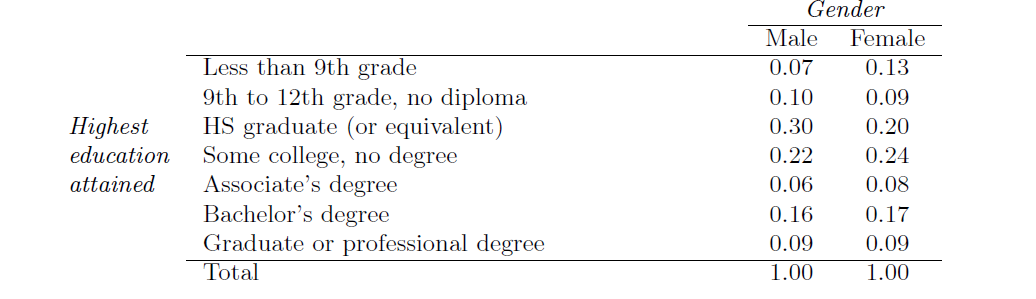
\includegraphics[width=.9\linewidth]{table.png}
\end{center}

\subsection{What is the probability that a randomly chosen man has at least a Bachelor's degree?}
\label{sec:org2822706}
It's \(0.16 + 0.09 = 0.25\).
\subsection{What is the probability that a randomly chosen woman has at least a Bachelor's degree?}
\label{sec:orgbda83d1}
It's \(0.17 + 0.09 = 0.26\).
\subsection{What is the probability that a man and a woman getting married both have at least a Bachelor's degree? Note any assumptions you must make to answer this question.}
\label{sec:org292a48b}
Assuming that both events are independent, if both of them should have at least a Bachelor's degree, we can just find the product of their individual probability: \(0.25 * 0.26 = 0.065\). 
\subsection{If you made an assumption in part (c), do you think it was reasonable? If you didn't make an assumption, double check your earlier answer and then return to this part.}
\label{sec:orgd6b18b5}
I don't think it's reasonable. We have to consider that many people get married with people they met while living similar experiences (high school/college dating, work environment, \ldots{}), therefore we should not expect that the events are independent, because they probably have the same education to begin with.
\section{\underline{School absences}}
\label{sec:orgaeac4e1}
Data collected at elementary schools in DeKalb County, GA suggest that each year roughly 25\% of students miss exactly one day of school, 15\% miss 2 days, and 28\% miss 3 or more days due to sickness.
\subsection{What is the probability that a student chosen at random doesn't miss any days of school due to sickness this year?}
\label{sec:org7488304}
The random student can't be in any of the sets described, so we have \emph{100\% - 25\% - 15\% - 28\% = 32\%}.
\subsection{What is the probability that a student chosen at random misses no more than one day?}
\label{sec:org18a9eca}
The random student, now, can fall into the 1st set presented, giving us \emph{100\% - 15\% - 28\% = 57\%}.
\subsection{What is the probability that a student chosen at random misses at least one day?}
\label{sec:org1c06628}
We can just take away the probability found in the 1st question, giving us \emph{100\% - 32\% = 68\%}.
\subsection{If a parent has two kids at a DeKalb County elementary school, what is the probability that neither kid will miss any school? Note any assumption you must make to answer this question.}
\label{sec:org5868862}
We must assume that the events are independent. This way, we can just simply find the product of the probabilities: \(0.32 * 0.32 = 0.1024\).
\subsection{If a parent has two kids at a DeKalb County elementary school, what is the probability that both kids will miss some school, i.e. at least one day? Note any assumption you make.}
\label{sec:org2564ecc}
We take the same assumption as before. Now we find \(0.68 * 0.68 = 0.4624\).
\subsection{If you made an assumption in part (d) or (e), do you think it was reasonable? If you didn't make any \assumptions, double check your earlier answers.}
\label{sec:org7847b57}
We have the same case as the previous question, in which people will frequent the same places. It's even clearer, in this example, that the events are not independent. Suppose one of the kids is sick, the other one might get sick because of it. Suppose that the parents are super neurotic and never get sick, both kids will frequent an establishment where getting diseases is hard. This way, we can conclude that the assumption isn't reasonable.
\end{document}
